% Griffin-Fp192 precompile AIR — multi-chip / cross-table-lookup architecture,
% in the style of Dokchitser-Bulkin "ZKVM step by step" (ePrint 2023/1032, Fig.1)
% and the SP1 chip model (ePrint 2025/2204): chips = witness tables; dashed = lookup;
% double = permutation. ALL columns are the REAL ones from
% docs/precompile_soundness/griffin_fp192.md (GriffinFp192Chip / ControlCols,
% InteractionKind::GriffinFp192 = 22, receive_syscall, 14 rows/syscall).
% Compile: pdflatex griffin_air_chips.tex
\documentclass[border=4pt]{standalone}
\usepackage{tikz}
\usepackage{newtxtext,newtxmath}
\usetikzlibrary{positioning,arrows.meta,fit,calc,matrix}
\begin{document}
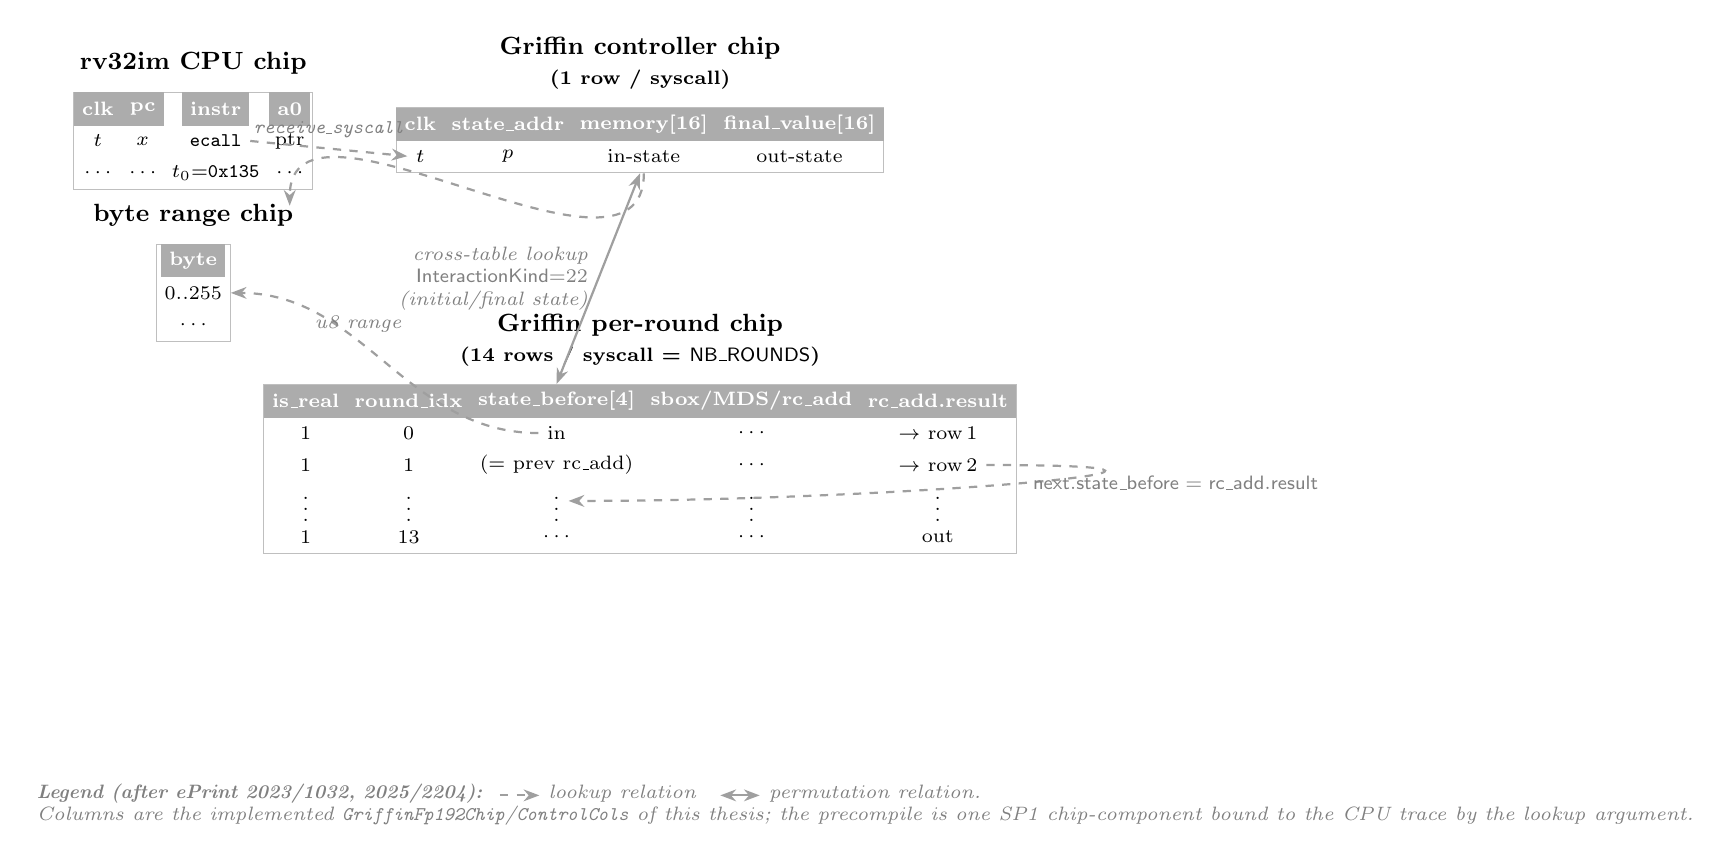
\begin{tikzpicture}[
  font=\small,
  >={Stealth[length=2mm]},
  tbl/.style={matrix of nodes, nodes={font=\scriptsize,minimum height=4.2mm,inner xsep=3pt,anchor=center},
              row 1/.style={nodes={fill=gray!65,text=white,font=\scriptsize\bfseries}},
              row sep=-\pgflinewidth, column sep=-\pgflinewidth,
              nodes in empty cells, draw=gray!50, inner sep=0pt},
  title/.style={font=\bfseries\small,align=center},
  look/.style={->,dashed,gray!75,thick},
  perm/.style={<->,gray!75,thick},
  cnote/.style={font=\scriptsize\itshape,gray},
]

% ===== rv32im CPU chip =====
\node[title] (cpuT) {rv32im CPU chip};
\matrix[tbl,below=1mm of cpuT] (cpu) {
  clk & pc & instr & a0 \\
  $t$ & $x$ & \texttt{ecall} & ptr \\
  $\cdots$ & $\cdots$ & $t_0{=}\mathtt{0x135}$ & $\cdots$ \\
};

% ===== Controller chip (1 row / syscall) =====
\node[title,right=22mm of cpuT] (ctrlT) {Griffin controller chip\\\scriptsize (1 row / syscall)};
\matrix[tbl,below=1mm of ctrlT] (ctrl) {
  clk & state\_addr & memory[16] & final\_value[16] \\
  $t$ & $p$ & in-state & out-state \\
};

% ===== Per-round chip (14 rows / syscall) =====
\node[title,below=26mm of ctrlT] (rndT) {Griffin per-round chip\\\scriptsize (14 rows / syscall = $\mathsf{NB\_ROUNDS}$)};
\matrix[tbl,below=1mm of rndT] (rnd) {
  is\_real & round\_idx & state\_before[4] & sbox/MDS/rc\_add & rc\_add.result \\
  1 & 0 & in & $\cdots$ & $\to$ row\,1 \\
  1 & 1 & (= prev rc\_add) & $\cdots$ & $\to$ row\,2 \\
  $\vdots$ & $\vdots$ & $\vdots$ & $\vdots$ & $\vdots$ \\
  1 & 13 & $\cdots$ & $\cdots$ & out \\
};

% ===== byte range-check (lookup target) =====
\node[title,below=12mm of cpuT,yshift=-2mm] (brT) {byte range chip};
\matrix[tbl,below=1mm of brT] (br) {
  byte \\ $0..255$ \\ $\cdots$ \\
};

% ===== arrows =====
% CPU ecall -> controller (syscall receive)
\draw[look] (cpu-2-3.east) -- node[cnote,above]{\texttt{receive\_syscall}} (ctrl-2-1.west);
% controller <-> per-round : cross-table LOOKUP (InteractionKind 22) = permutation of state limbs
\draw[perm] (ctrl.south) -- node[cnote,left,align=right,pos=0.5]{cross-table lookup\\$\mathsf{InteractionKind}{=}22$\\(initial/final state)} (rnd-1-3.north);
% per-round cross-row state threading (next.state_before = local.rc_add.result)
\draw[look] (rnd-3-5.east) to[out=0,in=0,looseness=2] node[cnote,right]{$\mathsf{next.state\_before}=\mathsf{rc\_add.result}$} (rnd-4-3.east);
% per-round bytes -> byte range chip
\draw[look] (rnd-2-3.west) to[out=180,in=0] node[cnote,above,pos=0.6]{u8 range} (br-2-1.east);
% memory binding controller -> CPU memory (dashed lookup)
\draw[look] (ctrl-2-3.south) to[out=270,in=90] ($(cpu-3-4.south)+(0,-2mm)$);

% ===== legend =====
\node[cnote,below=20mm of br.south,anchor=north west,align=left] (leg) at ($(rnd.south west)+(-30mm,-8mm)$)
  {\textbf{Legend (after ePrint 2023/1032, 2025/2204):}\ \ %
   \tikz[baseline]\draw[look](0,.4ex)--(5mm,.4ex);\ lookup relation\quad
   \tikz[baseline]\draw[perm](0,.4ex)--(5mm,.4ex);\ permutation relation.\\
   Columns are the implemented \texttt{GriffinFp192Chip}/\texttt{ControlCols} of this thesis; the precompile is one SP1 chip-component bound to the CPU trace by the lookup argument.};
\end{tikzpicture}
\end{document}
